\section{Proposed Methodology: SurroSelect}\label{sec:method}
\subsection{Overview}
SurroSelect takes the $N$ runs and returns (a) the selected stand-in, (b) the set of models tied with it, (c) a basis check, and (d) a learning-curve forecast (\cref{fig:framework}, \cref{alg:surroselect}). Every step uses only the training runs.
\begin{figure}[t]\centering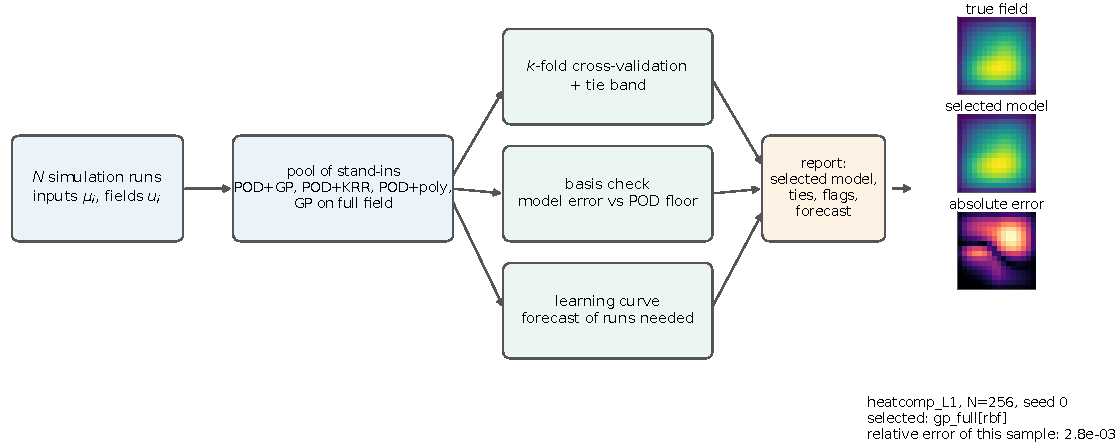
\includegraphics[width=\textwidth]{figures/fig_framework.pdf}
\caption{SurroSelect pipeline. The $N$ simulation runs enter a pool of stand-in models; $k$-fold cross-validation selects the best model and reports which others are tied with it; the basis check compares the model error with the error of projecting held-out fields onto the POD basis; the learning curve forecasts the error for more runs. The example fields are taken from the first test sample of problem \texttt{heatcomp\_L1} (seed~0, $N=256$): true field, selected model, and absolute error, as chosen by the rule in \cref{sec:qualitative}.}\label{fig:framework}\end{figure}

\subsection{Candidate pool}
The default pool has seven members, all classical: POD+GP with a Mat\'ern-5/2 kernel and rank 32, with a squared-exponential kernel and rank 32, and with Mat\'ern-5/2 and rank 8 (GP on the four leading modes with marginal-likelihood fitting, remaining modes sharing the fourth kernel); POD+KRR-wide, whose kernel, length-scale ($0.05$--$15\sqrt p$ on the unit box) and ridge ($10^{-16}$--$10^{-2}$ times $N$) are chosen over a wide grid by the leave-one-out error of \cref{prop:loo}; POD+polynomial, degree up to six with at most 3000 features, degree and ridge chosen by leave-one-out; and a GP directly on the full field (Mat\'ern-5/2 or squared-exponential, shared ARD kernel fitted on at most 300 runs), included only when $m\le2000$. A tuned neural network (\texttt{TunedMLP}, \cref{sec:setup}) can be added as an optional member.

\subsection{Cross-validated, tie-aware selection}
Each member is scored by $k$-fold cross-validation ($k=4$ by default) with all fitting, including hyper-parameter fitting, repeated inside each training fold. The member with the smallest mean cross-validated error~\eqref{eq:err} is selected, and all members within the tie band of \cref{sec:prelim} are reported as tied. Members that fail to fit receive infinite error.

\subsection{Basis check}
On each fold, a rank-32 POD basis is fitted on the training part and the held-out fields are projected onto it; the mean relative error of this projection is the \emph{basis floor}. If the best POD-based member's cross-validated error is within 25\% of the floor, the tool flags the basis as limiting and recommends a full-field model, a larger basis, or a nonlinear output map. The reason is \cref{prop:floor}.

\subsection{Budget forecast}
For the selected member, cross-validated errors are computed at 1/8, 1/4, 1/2 and all of the training folds. A power law $e(n)=A\,n^{-b}$ is fitted by least squares in log--log coordinates to the last three points (central forecast) and to all four (alternative); the lower and upper of the two forecasts form a range. The number of runs needed for a target error $\varepsilon$ is $(A/\varepsilon)^{1/b}$; the tool declines to answer if $b<0.1$ or if the answer exceeds sixteen times the current number of runs. This is an extrapolation and is validated in \cref{sec:results-tool}, not assumed.

\begin{algorithm}[t]\caption{SurroSelect (default settings)}\label{alg:surroselect}
\KwIn{runs $(\boldsymbol\mu_i,\mathbf u_i)_{i\le N}$, folds $k$, tie band $\tau=0.1$ decade, optional target error $\varepsilon$}
Scale inputs to the unit box; split the runs into $k$ folds\;
\ForEach{pool member $c$}{ fit $c$ on each training fold and score it on the held-out fold; $e_c\leftarrow$ mean error \eqref{eq:err}\;}
$c^\star\leftarrow\arg\min_c e_c$; tied set $\leftarrow\{c:\ e_c\le 10^{\tau}e_{c^\star}\}$; refit $c^\star$ on all $N$ runs\;
Basis floor $\phi\leftarrow$ mean projection error of held-out fields onto a rank-32 POD basis; flag the basis if $e_{c^\dagger}\le1.25\,\phi$ for the best POD-based $c^\dagger$\;
Learning curve: errors of $c^\star$ at $n\in\{N/8,N/4,N/2,N\}$ (training-fold sizes); fit $\log e=\log A-b\log n$ on the last three points (and on all four); forecast $e(4N)$; if $\varepsilon$ is given, return $(A/\varepsilon)^{1/b}$ unless $b<0.1$ or the result exceeds $16N$\;
\Return{$c^\star$, tied set, basis flag, forecast}
\end{algorithm}

\subsection{Theory}
Two results are standard and are included because the tool relies on them; proofs are in the Supplement (\cref{sec:S-proofs}).
\begin{proposition}[Closed-form leave-one-out]\label{prop:loo}
For a ridge smoother with hat matrix $H$ (so $\hat{\mathbf a}=H\mathbf a$ on the training inputs), the leave-one-out prediction error at run $i$ equals $(a_i-\hat a_i)/(1-H_{ii})$. For $H=K(K+\lambda N I)^{-1}$ with $K=Q\,\mathrm{diag}(w)Q^\top$, $1-H_{ii}=\sum_j Q_{ij}^2\,\lambda N/(w_j+\lambda N)$, which can be evaluated without cancellation when $\lambda N$ is tiny.
\end{proposition}
\begin{proposition}[Basis floor]\label{prop:floor}
Let $\hat{\mathbf u}$ be any model whose outputs lie in the affine subspace $\bar{\mathbf u}+\mathrm{span}(V_r)$. Then for every run, $\lVert\hat{\mathbf u}-\mathbf u\rVert_2\ge\lVert(I-V_rV_r^\top)(\mathbf u-\bar{\mathbf u})\rVert_2$, so the mean relative error of $\hat{\mathbf u}$ is at least the mean relative projection error of the basis, whatever the regressor.
\end{proposition}
The first is the PRESS identity for ridge regression~\cite{golub1979}; the second is the optimality of orthogonal projection. The forecast has no guarantee: it is exact only if the error follows a power law, and \cref{sec:results-tool} tests how often it is useful.
